\chapter{Background}
\renewcommand{\baselinestretch}{\mystretch}
\label{chap:Back}
%\setlength{\parindent}{0pt}
\PARstart{B}{ack} ground theory, related research and the existing tool will be provided in this chapter with a detailed illustration. The first section 2.1 will further describe how to find a trade-off among three mainstream model type: black box, grey box and white box. Following section introduce the tested HST: Berkeley design ABC with its highlights and innovative algorithms. In the final section, we will discuss the investigation and evaluation of existing fuzz testing tool in hardware synthesis: VlogHammer.
\section{Fuzz testing and model selection}
As mentioned before, fuzz testing was proposed by Dr.Barton Miller. Through 20 years of development, it has been widely applied in software validation and security testing area. Microsoft's Springfield Project offers fuzz testing service to the public. OSS-Fuzz Continue from Google provides fuzz testing for open-source projects. 
\subsection{Black-box fuzzing}
The Black-box fuzzing is a random testing method which only considers the correctness of the output result or function. The generation process of black-box fuzzing bases on its pre-defined input, called ''seeded input'' \cite{nidhra2012black}. The inside structure and operation principle of DUT are not concerned in this kind of test model.Fig \ref{fig:balckbox} shows the construction of the black-box model. 
\begin{figure}[htbp]
    \centering
    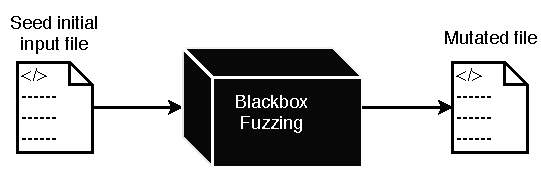
\includegraphics[width=10cm]{MScThesisTemplate/Figs/blackbox.pdf}
    \caption{\footnotesize Black-box fuzzing}
    \label{fig:balckbox}
\end{figure}

Mutation is an important characteristic of black-box fuzzing. With a valid seeded input, the output of the test generator can randomly mutate to other test-generation heuristics \cite{bounimova2013billions}. The DUT's bugs or vulnerabilities are expected to be evoked by the randomly generalised inputs. Black-box testing is a cost-effective method in finding bugs. According to the prescription of a multinational technology company like Microsoft \cite{bounimova2013billions}, black-box fuzzing is a compulsory procedure of every newly designed device or programmed software. It is known as "Security Development Lifecycle" \cite{howard2006security} in Microsoft product manual. However, the disadvantage of the black-box fuzzing is relative low code coverage and bug missing. The following short program provides an example. It shows that the probability of triggering the bug in conditional branch \texttt{then} is $1/2^{32}$, which is very low. Because \texttt{int} type is a 32-bit long parameter and only one corresponding number \texttt{2019} can induce the error issue.
\begin{lstlisting}[float=htb,
        label=lstcode,
        language=C++,
        basicstyle={\footnotesize\ttfamily},
        keywordstyle=\color{blue}, 
        commentstyle=\color{CPPGreen},
        escapeinside=``,
        %breaklines,
       xleftmargin=2em,xrightmargin=2em, aboveskip=1em,
        tabsize=4]
int fuzz(int x){
    int y = x + 1;
    if (y == 2019) 
        abort();//Bug location
    return 0;
}
\end{lstlisting}
\subsubsection{Csmith}
Csmith is a typical implementation of black-box fuzzing. As Yang et al. mentioned in their paper \cite{Yang:2011:FUB:1993316.1993532}, they designed Csmith as a "randomised test-case generation tool". The generated C programs by Csmith involve most kinds of C expressions and statements those were defined in the C99 standard. Other commonly-used features in C language such as control flow (\texttt{if/else},\texttt{for} loop, \texttt{break}), variable definition (\texttt{int},\texttt{char}), operation (arithmetic, logical and bitwise) are also covered by Csmith. The structure of the Csmith shows in Fig. \ref{Fig:csmith}. The test harness has been passed to three different compilers to execute it. Comparison among the three compilers' results, the minority indicates that it has a large probability of containing bugs or vulnerabilities. 

Avoiding inadequacies for the compilers, each generated program by Csmith has a unique interpretation. Csmith's C program generation follows top-down architecture. The global environment of Csmith describes the highest level of definitions. The local environment defines three information: current call chain, objects and all in-scope pointers \cite{Yang:2011:FUB:1993316.1993532}. Guided by probability table, the Csmith construct the c code file step by step from basic \texttt{main} to branch function and sub-objects. The researchers spent three years to find serves, previous unknown bugs in mainstream C compilers such as GCC, LLVM and other commercial tools. After three years of testing, the number of detected unknown bugs is 325. The detected bugs have been reported to the compiler developer.  The types of bugs involve compiler crash and returning wrong compiling output results \cite{klees2018evaluating}. The quantitative analysis of Csmith shows that the code coverage of Csmith is high in line testing (75.58\%) and function testing (82.41\%), but low in branch tesing (46.26\%).

Csmith proves that black-box fuzzing is a worth considering model in HST testing because of the impressive effectiveness of bug finding. It detected 325 unknown bugs in short three years. The design structure is easy to understand and implement.

\begin{figure}[htbp]
\centering
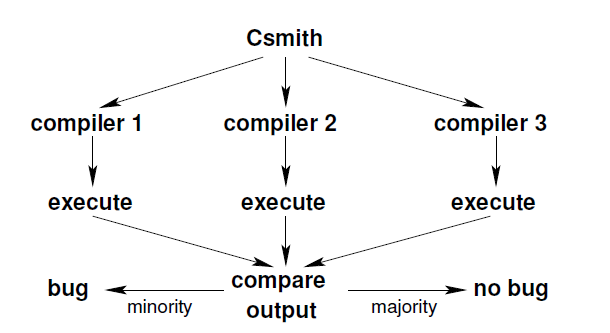
\includegraphics[scale=0.6]{MScThesisTemplate/Figs/Csmith.PNG}
\caption{\footnotesize Csmith architecture \cite{Yang:2011:FUB:1993316.1993532}}
\label{Fig:csmith}
\end{figure}

\subsection{White-box fuzzing}
White-box fuzzing is an alternative fuzz testing method. With the development of systematic dynamic test generation \cite{godefroid2005dart}, the white-box fuzzing has been extended from unit-level to integrated system level. The white-box fuzzer will dynamically operate the symbolic executed input until all feasible path of the DUT has been swept. Testing structure of the white-box fuzzing shapes like a "Tree" ( in Fig.\ref{fig:whitebox}). Using above program in \ref{lstcode} as example, the initial seed value of input \texttt{x} is \texttt{1} and \texttt{y = x + 1} which will assign \texttt{2} to \texttt{y}. The path constrain \texttt{2} $\neq$ \texttt{2019} yields the execution of conditional branch \texttt{else}. Following the execution of one conditional branch under such constraint, the next input would be \texttt{x = 2018} to allow the execution of the other conditional branch. The input format and specifications do not need to know. Moreover, each path of the DUT and internal perspective of the DUT will be egoistic tested. It ensures the high code coverage of white-box fuzzing \cite{functest}.

Compared with black-box fuzzing, white-box fuzzing has an advantage in full path thorough testing. The testing processes are traceable and easy to automate. In practice, a large number of paths can not be precisely tested within a reasonable time. Besides, white-box fuzzing increases the complexity of testing and reduce the universality. Therefore, the design of white-box fuzzer might be closely related to the specific implementation of DUT. Rewriting the output generated by designed fuzzer may lead to assumption failure or occur unnecessary error \cite{nidhra2012black}\cite{bounimova2013billions}. Moreover, white-box fuzzing costs too much computational resource in dynamic symbolic execution. 

\begin{figure}[htb]
    \centering
    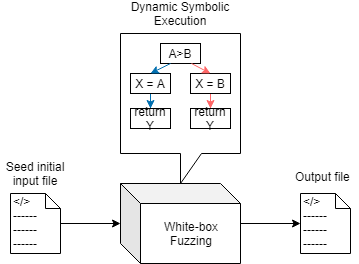
\includegraphics[width=10cm]{MScThesisTemplate/Figs/whitebox.pdf}
    \caption{\footnotesize White-box fuzzing}
    \label{fig:whitebox}
\end{figure}
\subsubsection{SAGE}
In Bounimova et al.'s paper \cite{bounimova2013billions}, they proposed a constraint-based white-box fuzzer SAGE. The developers aim to generate large numbers of instruction and statements in single symbolic execution. Thus, the generational search strategy of the SAGE was creative and innovative. The first step of symbolic execution is to create a path constraint. The rest of the constraints in this path will be solved by a constraint solver and ''placed in conjunction with the prefix of the path constraint leading to it'' \cite{bounimova2013billions}. The static result shows that single execution can generate 25,598 full path constraints.

Fig \ref{Fig:sage} shows the structure of SAGE. An initial input would be passed to SAGE to run the program test. If the program crashes, it means that this initial input may trigger a bug. If not, the SAGE will symbolically execute the program with that input and generate the required path constraints. When the constraints solver has solved all the constraints in that path, the satisfied constraints would be mapped into \texttt{N} different inputs to improve the instruction coverage. \texttt{N} constrains would be ranked in terms of the ability to discover new instructions. The next symbolic execution of SAGE will adopt the highest mark input as its input \cite{bounimova2013billions}.

The result of SAGE shows that the SAGE fuzzer can find around 50 unique bugs in 23 days of running it on 200 programs. Compared with the bug hunting ability of the black-box model (352 bugs in three year's testing), the efficiency has been greatly improved. It proves the advantage of white-box in high code coverage and full path-through testing. However, the implementation of SAGE uses dynamic systematic generation execution. The structure diagram of SAGE (Fig \ref{Fig:sage}) is much more complicated than the black-box fuzzer Csmith \ref{Fig:csmith}). 
\begin{figure}[htb]
\centering
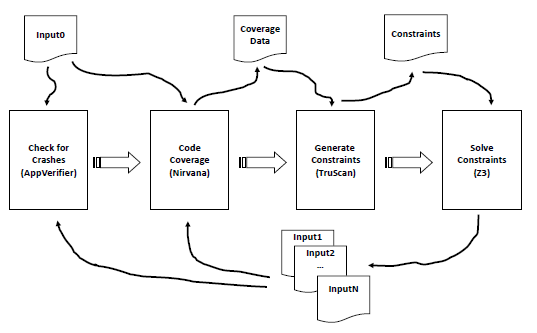
\includegraphics[scale=0.9]{MScThesisTemplate/Figs/sage.PNG}
\caption{\footnotesize SAGE architecture\cite{bounimova2013billions}}
\label{Fig:sage}
\end{figure}

\subsection{Tradeoff: Grey-box fuzzing}
Leveraging the pros and cons of black-box fuzzing and white-box fuzzing, this project decided to use the intermediate model: grey-box fuzzing model. Grey-box fuzzing integrates the features of black-box and white-box. It partly knows the inside structure, code and algorithm of DUT. However, the test aim is to check the correctness of output result. 

Greybox fuzzing is beneficial in HST testing. A tailored mutation for HST has better bug-finding efficiency than pure mutation.  Because some test cases generated by pure mutation may be repetitive and can not trigger the corner cases or malicious behaviours.  Having some knowledge of the HST is important due to its requirement of input file format. For example, if the generated HDL file has a \texttt{alwasy @(posedge CLK or negadge RST)} structure, to separate the signals in sensitive list, it may also use ''\texttt{,}'' instead of ''\texttt{or}''. The latest standard Verilog 2001 \cite{ieee2001} supports this replacement, but some synthesis tools they parse input based on older standard Verilog 1995 can not yield a synthesised netlist and regard it as a syntax error. In addition, the output netlist of DUT not only expected to correct execution but also expected to be synthesised in an optimised way. For instance, two inverters, two AND gates and an OR gate are connected in Fig \ref{fig:circuitoptim}'s way. After circuit optimising, it could be represented by single XOR gate \cite{mano2015logic}. It is difficult and unnecessary to test all this detail synthesis procedure. Gery-box's results targeted provide flexibility and efficiency in fuzzer design. We do not need to focus on testing each path of the synthesis..
\begin{figure}[htbp]
    \centering
    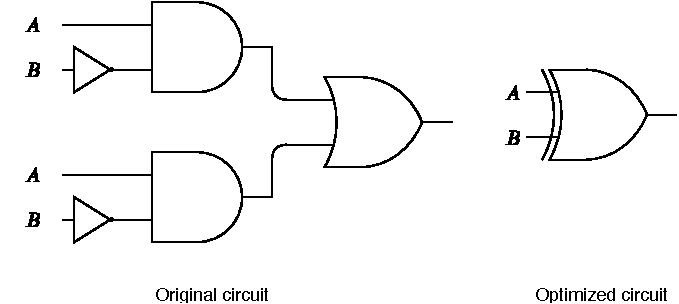
\includegraphics[scale=0.8]{MScThesisTemplate/Figs/circiut_opti.pdf}
    \caption{\footnotesize Circuit optimisation}
    \label{fig:circuitoptim}
\end{figure}
Conventionally, the generation of grey-box fuzzing need a feedback loop to guided the next seed. Following Fig \ref{fig:gerybox} shows the architecture of grey-box fuzzing. Execute condition of the feedback loop is decided by some metrics for example, label coverage \cite{havrikov2017sym,havrikov2017efficient}, branch distance \cite{havrikov2017efficient}. The feedback-driven fuzzer can leverage input and execution towards the testing aims. The detail part of this projects fuzzer will be presented in the methodology section of Chapter 3.
\begin{figure}[htbp]
    \centering
    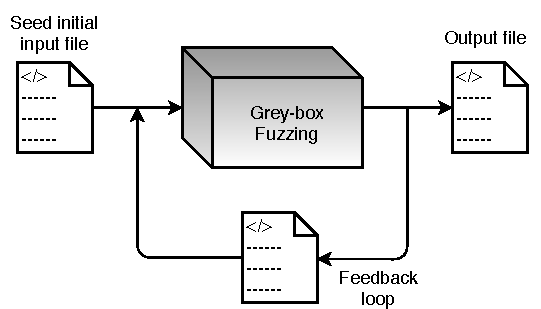
\includegraphics[scale=0.8]{MScThesisTemplate/Figs/greybox.pdf}
    \caption{\footnotesize Grey-box fuzzing}
    \label{fig:gerybox}
\end{figure}
\section{Hardware synthesis: Berkeley designed ABC}
ABC is a powerful synthesis and formal verification tool in hardware designs. It was developed by Robert Brayton and Alan Mishchenko in University of California, Berkeley. Since 2005, ABC has been gaining momentum and attention to be a ''public-domain'' tool in hardware logical synthesis and verification \cite{ABC}. In this project, ABC was used as a synthesis tool. As a result, the verification function of ABC was neglected. Figure \ref{fig:abc_fun} display the interactions and functions of ABC.
\begin{figure}[htbp]
    \centering
    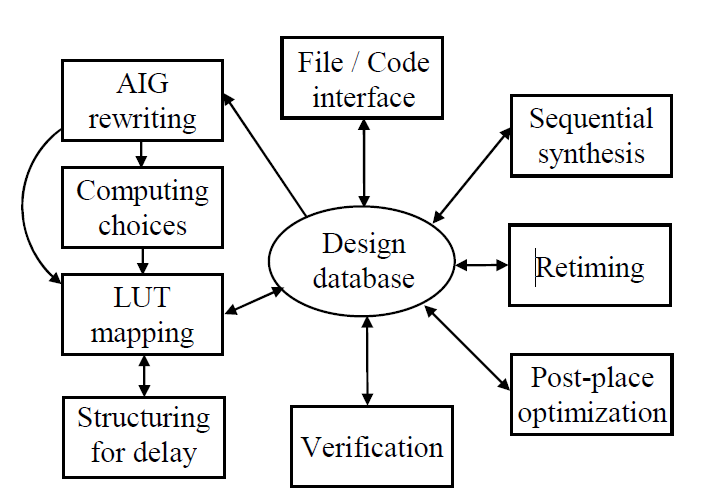
\includegraphics[scale=0.6]{MScThesisTemplate/Figs/abc_fun.PNG}
    \caption{\footnotesize Interactions and functions of ABC \cite{ABC}}
    \label{fig:abc_fun}
\end{figure}

\subsection{Selection motivation}
The first reasons for selecting ABC as a DUT is that ABC occupies a dominant position in academic research. ABC has been widely used by the University of Colorado (Boulder), Cornell University and University of California (Berkeley). If a bug or Vulnerability was found in the ABC, it is beneficial for the academic staff to avoid wrong scientific research. 

Secondly, the open-source feature of ABC is significant merit. As an open-source tool of Electronic Design Automation(EDA), ABC is source code can be forked from Github \url{https://github.com/berkeley-abc/abc}. Developing in open-source mode can improve the software's reliability due to the contribution of thousands of independent programmers in software testing and bugs fixing.\cite{laurent2004understanding} With the source code of ABC, the design of the fuzz testing could use the grey-box fuzzing model. As discussed in the above section, no doubt that the designed testing tool will be more efficient and pertinence. Besides, the access to viewing and modifying source code of ABC allow us to inject bugs to ABC in future analysis.

The third reason for select ABC is its high efficiency. The synthesis method of ABC has been switched from multi-level valued to binary And-Inverter Graphs (AIGs). The following figure \ref{fig:abc_aig} show the principle of the AIG synthesis with Karnaugh map and Boolean expression. Comparing to its predecessor SIS (developed by the research group of UC Berkeley in 1987-1991\cite{ABC}), it saves the runtime and memory space. The scalability of ABC has increased due to the saving in the above two aspects.
%%%%%%%%%%%%%%%%%%%%%%%%%%%%%
\begin{figure}[htbp]
    \centering
    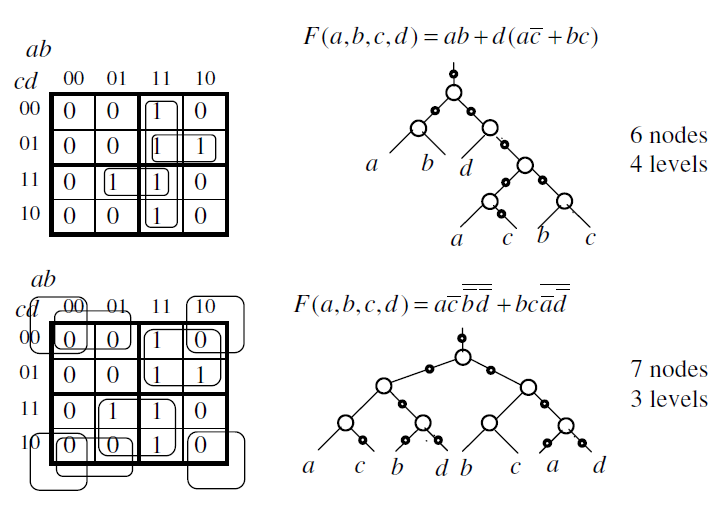
\includegraphics[scale=0.6]{MScThesisTemplate/Figs/abc_aig.PNG}
    \caption{\footnotesize AIG generation of ABC\cite{mishchenko2006dag}}
    \label{fig:abc_aig}
\end{figure}
In addition, ABC attached equivalence checker provided an efficient way in the final comparison stage of this project. It could handle both combinational and sequential circuit based on SAT sweeping \cite{satsweep,kuehlmann2001circuit,mishchenko2006improvements}. Two circuits will be transformed into a mitre which is consisted of XOR gates and OR gates. The inputs of the original circuit will be transmitted to XOR gates and ORed to yield an output of the mitre. This equivalence checker has been awarded two out of three categories at hardware model checking competition at CAV 2008. It certified that the checking result of the equivalence checker is reliable \cite{mishchenko2006improvements}.

\subsection{Highlights and commands}
HST is expected to convert a high-level HDL into an optimised gate-level representation (netlist). The transformation needs to satisfy some criteria such as optimise the gate number, logic level and node number. The important functions of ABC are: it combines logic circuit optimisation, effective mapping for cells and look-up tables and creative synthesis of sequential circuit \cite{ABC}.

\textbf{Multiple in-out parse:} Different format input files can be parsed by ABC. Its manual shows that binary BLIF \cite{blif} (\texttt{.blif}), AIG (\texttt{.aig}), BENCH (\texttt{.bench}), Synopsys equation \cite{Synopsys} (\texttt{.eqn}) and Verilog (\texttt{.v}) can be read by ABC and converted to required format. With the help of ABC's multiple in-out parse, other synthesis tools those do not support Verilog format could be involved to enhance the final equivalence check (EC).

\textbf{Visualisation results:} For the synthesised netlist, ABC could output its structure in DOT file. Using graph visualisation package \href{https://www.graphviz.org}{GraphViz}, it can be transform into PNG format and offer intuitions. The visualisation function of ABC is beneficial to manual check of the output netlist structure of this project. A Verilog full adder module given as a sample input to show the visualisation results of ABC's circuit optimisation in Fig \ref{Fig.full} and \ref{Fig.full_b}. Other circuit optimisation command's visualisation result will be displayed in Appendix \ref{App:abc}.
%Need figure of execution
\begin{figure}[htb]
\centering
\subfigure[Verilog full adder]{
\label{Fig.full}
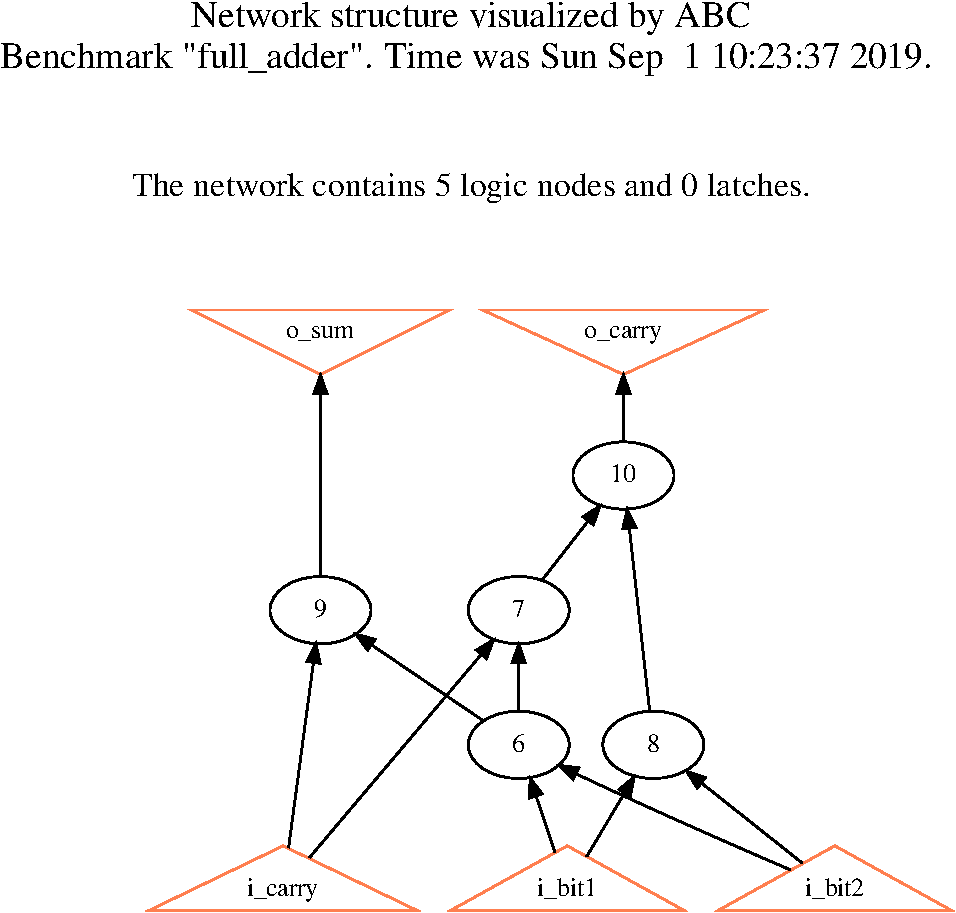
\includegraphics[width=0.45\textwidth]{MScThesisTemplate/Figs/full.pdf}}
\subfigure[Balanced circuit of ABC]{
\label{Fig.full_b}
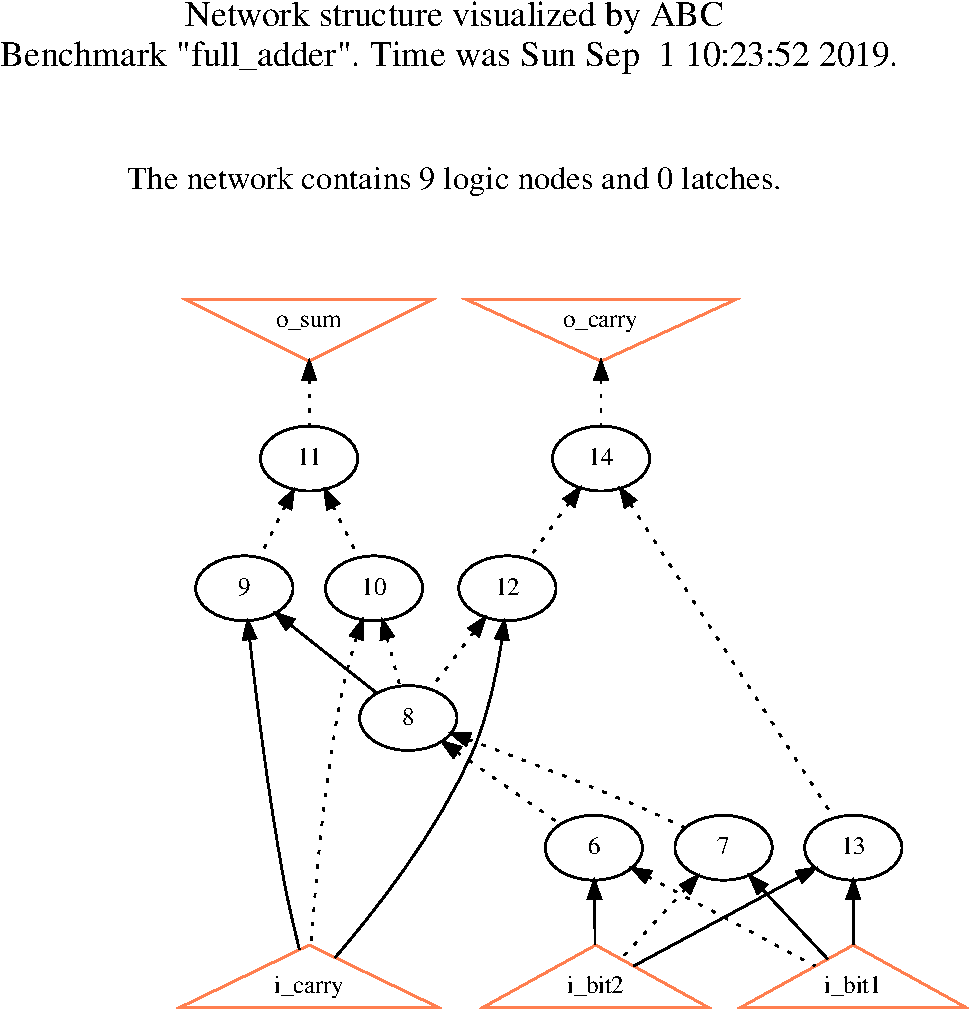
\includegraphics[width=0.45\textwidth]{MScThesisTemplate/Figs/full_b.pdf}}
\caption{\footnotesize Visualisation result of ABC}
\end{figure}

\textbf{Circuit optimisation:} ABC provide different circuit optimisation targeting sequential and combinational circuits. These optimisations can reduce circuit level, remove dangling nodes, remove latches and even carry structural hashing. The synthesised circuit become more compact and uniform. Thus, it improves the performance of the synthesised circuit and provides more measurable indicators of this project. 

The following table \ref{tab:command} shows the main ABC instructions involved in this project. Visual

\begin{table}[htb]
    \centering
    \begin{tabular}{c|c|m{8cm}}
        \hline
       \textbf{Command type} & \textbf{Command name} & \textbf{Function}\\
        \hline
     \multirow{3}{*}{Synthesis}&\textbf{\texttt{balance}} & ABC will automatically creates an equivalent circuit which has the minimum delay in two-input AND-gates (AIG format). The inverters do not influence the number of logic levels but the delay will be decrease due to the topological order tree-decomposition. \\
     \cline{2-3}
     & \textbf{\texttt{strash}}& The circuit will be transformed into an AIG through one-level structural hashing. As a purely combinational operation, the latches' property (position or number) will not be modified.\\
     \cline{2-3}
     & \textbf{\texttt{cycle}}& Random inputs will be provided to current sequential circuit to updates its state.\\
     \hline
     \multirow{2}{*}{Read}&\textbf{\texttt{read\_verilog}}& Parses the input file in Verilog which based on IWLS 2002 Benchmarks and  IWLS 2005 Benchmarks. \\
     \cline{2-3}
     & \textbf{\texttt{read\_blif}} & Pasee the input file in Berkeley Logic Interchange Format (BLIF) (compact and has short reading/writing times).\\
     \hline
     \multirow{2}{*}{Write}&\textbf{\texttt{write\_verilog}}& Outputs the network using technology independent Verilog.\\
     \cline{2-3}
     & \textbf{\texttt{write\_blif}}& Outputs the network in BLIF.\\
     \hline
\end{tabular}
    \caption{\footnotesize Main commands related in this project\cite{manual2006quick}}
    \label{tab:command}
\end{table}



\section{VlogHammer}
VlogHammer is a current existing regression tester to verify the circuit correctness of the Yosys's Verilog synthesis \cite{wolf2016yosys}. As Clifford (developer of VlogHammer and Yosys) discussed in VlogHammer's report \cite{wolf2016yosys}, it combines the auto-generated test case with the hand-written case. As a powerful tester VlogHammer can generate different types of the combinational logic circuit in Verilog and provide a detailed report. There are five procedures of VlogHammre: Test case generation, synthesis, checking, report generation and summary report. 

The fuzz testing algorithm used by VlogHammer is based on divide-and-conquer. The Fig \ref{fig:flowchart} shows the flowchart of Vloghammer. The boolean satisfiability (SAT) solver of Yosys is used to verify the synthesis results against original input Verilog file and coarse-grain RTL netlist synthesised by itself \cite{clifford,wolf2016yosys}.

Obtained from the test reports formed by VlogHammmer, Yosys and other third-party synthesis tools (used in comparison EC) were detected a couple of bugs. It interprets that synthesis of Verilog expressions in not particularly tricky of the tool, but it is hard to correctly synthesis all corner cases \cite{clifford}. An example test report shows in following table \ref{tab:Vloghammer}. Altera Quartus II and Xilinx ISIM separately produced incorrect synthesis results and simulation results. However, Modelsim simulates the resistor–transistor logic (RTL) netlist correctly. To identify the source of the bus, Modelsim was regarded as a reference to produce test cases and test benches. Verifying the synthesis results using Modelsim could avoid incorrect synthesis. Comparing the results produced by ISIM and Modelsim could distinguish whether there is a bug in ISIM.

\begin{table}[htb]
    \centering
    \begin{tabular}{c|ccccccc}
    \hline
         &\texttt{Vivado}& \texttt{Quartus}&\texttt{Xst}&\texttt{Yosys}&\texttt{Isim}&\texttt{Modelsim}&\texttt{Yosim} \\
         \hline
      \texttt{Vivado}&PASS&FAIL&PASS&PASS&d27539f3&d27539f3&d27539f3\\
      \texttt{Quartus}&FAIL&PASS&FAIL&FAIL&3ebd62e&3ebd62e&3ebd62e\\
      \texttt{Xst}&PASS&FAIL&PASS&PASS&d27539f3&d27539f3&d27539f3\\
      \texttt{Yosys}&PASS&FAIL&PASS&PASS&d27539f3&d27539f3&d27539f3\\
      \texttt{RTL}&PASS&FAIL&PASS&PASS&5a96447c&d27539f3&d27539f3\\
      \hline
    \end{tabular}
    \caption{\footnotesize VlogHammer's report\cite{clifford}}
    \label{tab:Vloghammer}
\end{table}
